\section{Performance and Discussion}
\subsection{Timings - Getting up to speed}
\begin{center}
    \begin{tabular}{|c|c|c|c|c|}
        \hline
        Version & -OO & -O3 & -Ofast -march=native & -O4\\
        \hline
        V1.1 & 24.304349 & 13.470492 & 12.901046 & 13.474097\\
        V1.2 & 24.204505 & 2.549037 & 2.035497 & 2.542937\\
        V1.3 & 12.155917 & 2.900762 & 2.836586 & 2.902077\\
        \hline
    \end{tabular}
\end{center}
Since the functions are now spread over several files, we need to check that we have as efficient timings as in the version without the Barnes Hut algorithm. To test this, we first use a check file to make sure our results are accurate. The timing results of this we omit.

The next step is to then compare timing results to that of previous results we have obtained.

Version 1.1 above is based on previous results from which we can compare. This involves using 3000 particles and 100 time steps. For this version (1.1) we have the functions \verb|r_vector|, norm and norm3 in the file vector.c, with the force functions from a previous version now in the forces.c file and all are called to the galsim.c main file. This shows some significant loss in computation time compared to a previous version. We now take all the vector functions into the forces.c file to see if this helps with computation time.

The next version (1.2) does indeed appear to speed up the computation times significantly for the flags apart from -O0.

Finally, in version (1.3), we make a comparison with the quadtree implemented for 3000 particles and 100 time steps to see how this compared. Before testing this, we ran this with $\theta$ set to zero first to ensure we maintained accuracy before optimising for $\theta$. This is allowed an accuracy of up to $10^{-3}$. The optimal value we obtained for $\theta$ is 0.25. This ran only marginally slower for all the flags apart from -O0, where this ran twice as fast.
\subsection{Timings - Which section to focus on}
Before we begin optimisation of the code, we look to which part of the code requires the most optimisation. We split the code into computing quadtree build time and forces computation time. We focused on the -Ofast and -march=native optimisation flags. The quadtree took 0.144213 seconds to compute for 5000 particles with 100 time steps. The forces took 5.302154 seconds to compute with the same parameters. On this evidence, we will look to focus our optimisations on computing the forces, since this took approximately $97\%$ of the computation time.
\subsection{Timings - Optimised}
\begin{center}
    \begin{tabular}{|c|c|c|c|c|}
        \hline
        Version & -OO & -O3 & -Ofast -march=native & -O4\\
        \hline
        V2.1 & 23.720430 & 5.669060 & 5.449106 & 5.842755\\
        \hline
        V2.2 & 23.545072 & 5.277797 & 4.420938 & 5.303275\\
        \hline
        V2.3 & 18.177161 & 5.102843 & 4.393660 & 5.105376\\
        \hline
        V2.4 & 17.941679 & 4.841763 & 4.289874 & 4.820603\\
        \hline
    \end{tabular}
\end{center}
Version 2.1 here involves having all the function calls in forces aside from \verb|vector_in_box|, which has been left out in the \verb|box_bounds.c| file.

This is where our first optimisation is. In Version 2.2, we chose to move \verb|vector_in_box| in to the forces file. This does indeed speed up the computation times for all apart from the -O0 flag.

In Version 2.3, we made an optimisation involving making a modification to \verb|theta_bounds|, which in turn meant we would have to make a modification to \verb|quad_force|. We took in two extra arguments in \verb|theta_bounds|, where we take pointers so that we only have to compute norm(r) just the once. This has some computational time effects for each flag, but mostly -O0.
\begin{center}
    Version 3 - \verb|theta_bounds|
\end{center}
\begin{lstlisting}{language=C}
    int theta_bounds(quadtree_t* tree, particle_t particle, double theta_max, vector_t* r, double* n) {
    double xwidth = tree->box.xupper - tree->box.xlower;
    *r = r_vector(tree->centre_of_mass, particle.position);
    *n = norm(*r);

    if(xwidth / *n < theta_max) {
        return 1;
    }
    else {
        return 0;
    }
}
\end{lstlisting}

In version 2.4, the final optimisation involved using our final \verb|theta_bounds| function, where we switched from dividing to multiplying. We did this since dividing is computationally more expensive than multiplying. This made for a minimal increase in performance on all the flags.
\begin{center}
    Version 4 - \verb|theta_bounds|
\end{center}
\begin{lstlisting}{language=C}
    int theta_bounds(quadtree_t* tree, particle_t particle, double theta_max, vector_t* r, double* n) {
    *r = r_vector(tree->centre_of_mass, particle.position);
    *n = norm(*r);

    return tree->box.xupper - tree->box.xlower < theta_max * (*n);
}
\end{lstlisting}
\begin{figure}[htb]
    \begin{center}
        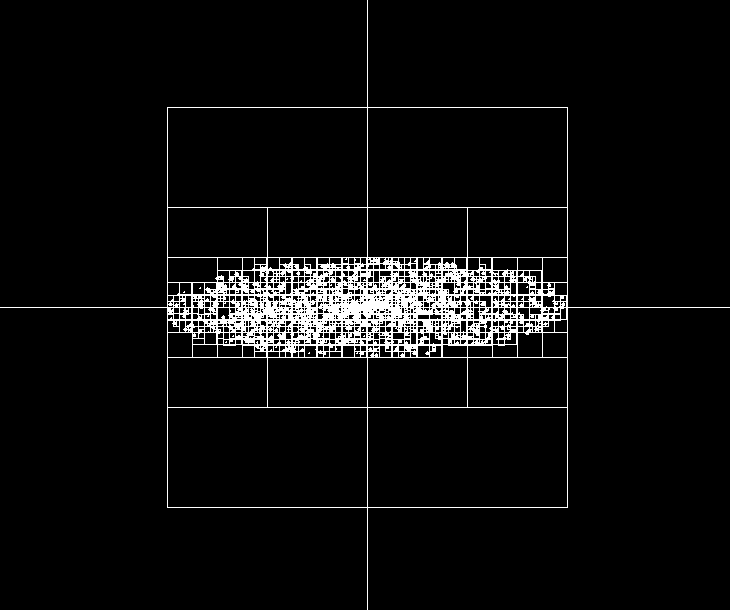
\includegraphics[width = 10cm]{../images/squarespace.png}
        \caption{A simulation of a galaxy}
    \end{center}
\end{figure}
\newpage
\subsection{Unsuccessful Optimisations}
We tried a few more optimisations on top of the ones described above, however, these were unsuccessful.

The first of these optimisations was to bring the forces.c file into the galsim.c file to see if there could be further time reductions in computation time. When this didn't produce any better time performance we decided to also bring in the quad.c file into the galsim.c file so that they are all located in the same place. Both were unsuccessful optimisations.
\subsection{Optimisation - Pthreads}
Since we saw from the previous section that the majority of computation time (approximately $95\%$) is spent computing the forces, we parallelize the code using pthreads in this part of the code.

Instead of computing the forces in a for loop on one thread, we have modified the code here to have a function point to all the relevant details of the particles updated. This function also included a start and stop point to compute forces given that we want to run certain sections of code on different threads.

To make sure this all runs fine, we need to include -pthread in the CCFLAGS.

We have the original problem size of 5000 particles and 100 time steps as one example and then 20000 particles with 200 time steps to see the potential speedup.
\begin{lstlisting}{language=C}
    typedef struct quad_force_args {
    quadtree_t* tree;
    particle_t* particles;
    double theta_max;
    vector_t* forces;
    int start;
    int stop;
} quad_force_args_t;

    void* quad_force_wrapper(void* argument) {
    quad_force_args_t* args  = argument;

    for(int i = args->start; i < args->stop; i++) {
        args->forces[i] = quad_force(args->tree, args->particles[i], args->theta_max);
    }

    return NULL;
}
//===========================================================================
void compute_quad_forces(vector_t* forces, quadtree_t* tree, particle_t* particles, int N, double theta_max, int nthreads) {

    pthread_t* thread_ptr = malloc(nthreads*sizeof(pthread_t));
    quad_force_args_t* args = malloc(nthreads*sizeof(quad_force_args_t));

    for(int i = 0; i < nthreads; i++) {
        args[i].tree = tree;
        args[i].particles = particles;
        args[i].theta_max = theta_max;
        args[i].forces = forces;
        args[i].start = (i * N) / nthreads;
        args[i].stop = ((i + 1)*N) / nthreads;
        pthread_create(&thread_ptr[i], NULL, quad_force_wrapper, &args[i]);
    }

    for(int i = 0; i < nthreads; i++) {
        pthread_join(thread_ptr[i], NULL);
    }
}
\end{lstlisting}
\newpage
\begin{figure}[htb]
    \begin{center}
        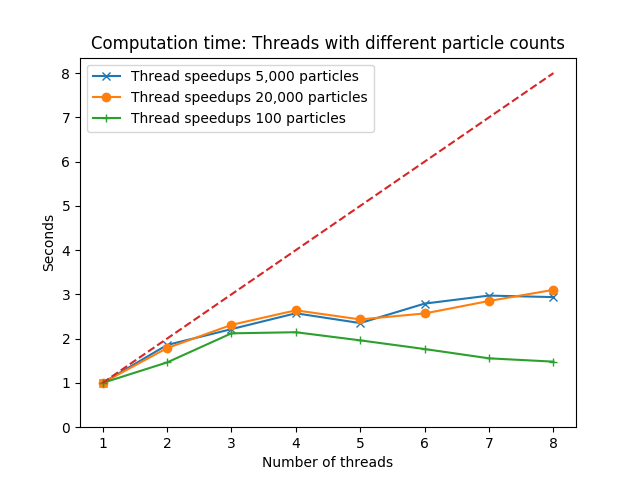
\includegraphics[width = 10cm]{../images/compute_times.jpg}
        \caption{Computation Times}
    \end{center}
\end{figure}
As we can see, larger files definitely benefit from extra cores at their disposal. Smaller files do not seem to require this, to the point where performance is actually reduced. The large difference in performance to ultimate best use is likely down to not having the 8 cores in which we can optimise with.
\subsection{Complexity}
Finally, below we have a plot outlining the computation times measured against $O(Nlog(N))$.
\begin{figure}[htb]
    \begin{center}
        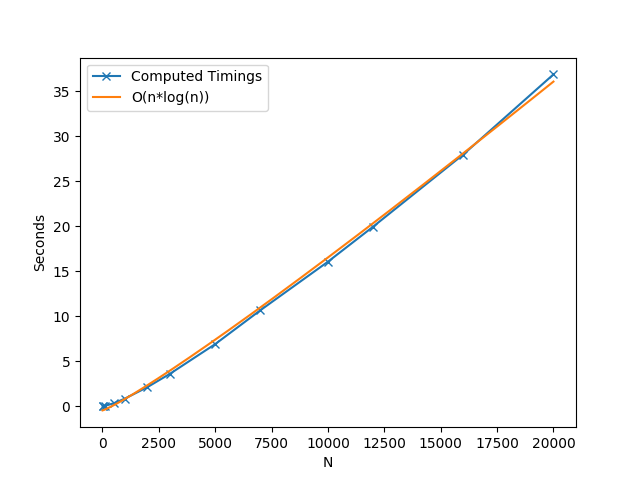
\includegraphics[width=14cm]{../images/nlogn.jpg}
        \caption{Time Complexity Plot}
    \end{center}
\end{figure}
